\chapter{集合}\label{ch16}

\emph{We all behave like Maxwell’s demon. Organisms organize. In everyday experience lies the reason sober physicists across two centuries kept this cartoon fantasy alive. We sort the mail, build sand castles, solve jigsaw puzzles, separate wheat from chaff, rearrange chess pieces, collect stamps, alphabetize books, create symmetry, compose sonnets and sonatas, and put our rooms in order, and all this we do requires no great energy, as long as we can apply intelligence.}

\begin{flushright}
    ——James Gleick, The Information: A History, a Theory, a Flood
\end{flushright}

Rust标准库里包含几种\emph{集合(collection)},它们是在内存中存储数据的泛型类型。我们已经在本书的很多地方使用过集合,例如\texttt{Vec}和\texttt{HashMap}。在本章中,我们将详细介绍这两种类型的方法,以及其他六种标准集合。但在我们开始之前,让我们先讨论一下Rust的集合和其他语言中的集合的一些不同之处。

首先,移动和借用无处不在。Rust使用移动来避免深拷贝。这就是为什么\texttt{Vec<T>::push(item)}方法以值获取参数,而不是以引用。值会被移动进vector。\hyperref[ch04]{第4章}中的图展示了实践中的表现:在Rust中把一个\texttt{String}添加到\texttt{Vec<String>}中很快,因为Rust不需要拷贝字符串的字符数据,字符串的所有权归属也总是很清楚。

其次,当集合改变大小或者被修改的同时还有指向它们的数据的指针时,Rust不会有无效性错误——即悬垂指针。无效性错误是C++中另一种未定义行为的来源,即使在内存安全的语言中也可能导致\texttt{ConcurrentModificationException}。Rust借用检查器会在编译器检查出它们。

最后,Rust没有\texttt{null},因此我们将在其他语言中需要\texttt{null}的地方看到\texttt{Option}。

除了这些不同之外,Rust的集合可能正是你需要的。如果你是经验丰富的程序员并且时间不多,你可以跳过这部分,但不要跳过“\nameref{entry}”。

\section{概述}

\autoref{t16-1}展示了Rust的8种标准集合。它们都是泛型类型。

\begin{table}[htbp]
    \centering
    \caption{标准集合总结}
    \label{t16-1}
    \begin{tabular}{p{0.2\textwidth}p{0.2\textwidth}lll}
        \hline
        \multirow{2}{*}{\textbf{集合}}  & \multirow{2}{*}{\textbf{说明}} & \multicolumn{3}{l}{\textbf{其他语言中的类似集合类型}} \\
        \cline{3-5}
         & & \textbf{C++} & \textbf{Java} & \textbf{Python} \\
        \hline
        
        \texttt{Vec<T>} & 可增长的数组  & \texttt{vector} & \texttt{ArrayList} & \texttt{list}  \\
        \rowcolor{tablecolor}
        \texttt{VecDeque<T>} & 双端队列(可增长环形缓冲区) & \texttt{deque} & \texttt{ArrayDeque} & \texttt{collections.deque} \\
        \texttt{LinkedList<T>} & 双向链表 & \texttt{list} & \texttt{LinkedList} & —— \\
        \rowcolor{tablecolor}
        \texttt{BinaryHeap<T> where T: Ord} & 大顶堆 & \texttt{priority\_queue} & \texttt{PriorityQueue} & \texttt{heapq} \\
        \texttt{HashMap<K, V> where K: Eq + Hash} & 键值哈希表 & \texttt{unordered\_map} & \texttt{HashMap} & \texttt{dict} \\
        \rowcolor{tablecolor}
        \texttt{BTreeMap<K, V> where K: Ord} & 有序键值表 & \texttt{map} & \texttt{TreeMap} & —— \\
        \texttt{HashSet<T> where T: Eq + Hash} & 基于哈希的无序集合 & \texttt{unordered\_set} & \texttt{HashSet} & \texttt{set} \\
        \rowcolor{tablecolor}
        \texttt{BTreeSet<T> where T: Ord} & 有序集合 & \texttt{set} & \texttt{TreeSet} & —— \\
    \end{tabular}
\end{table}

\texttt{Vec<T>}、\texttt{HashMap<K, V>}、\texttt{HashSet<T>}是最常用的集合类型。其他的集合都有适用的场景。这一章将轮流讨论每一个集合类型:

\codeentry{Vec<T>}
\hangparagraph{一个客增唱的、在堆上分配的、\texttt{T}类值的数组。本章中大约一半的篇幅专门介绍\texttt{Vec}和它的有用的方法。}

\codeentry{VecDeque<T>}
\hangparagraph{类似于\texttt{Vec<T>},但是用作先进先出队列会更好。它支持高效地在首部和尾部添加或移除元素,但这种能力的代价是其他操作会稍微慢一点。}

\codeentry{BinaryHeap<T>}
\hangparagraph{一个优先队列。\texttt{BinaryHeap}中的值按照一定结构组织,因此总是可以高效地找到和移除最大值。}

\codeentry{HashMap<K, V>}
\hangparagraph{一个键值对的表。通过键查找值很快速。表中的条目以任意顺序存储。}

\codeentry{BTreeMap<K, V>}
\hangparagraph{类似于\texttt{HashMap<K, V>},但按键的顺序保持条目有序。一个\texttt{BTreeMap<String, i32>}按照\texttt{String}的比较顺序存储条目。除非你需要条目保持有序,否则\texttt{HashMap}会更快。}

\codeentry{HashSet<T>}
\hangparagraph{类型\texttt{T}的值的集合。添加和删除元素都很快,查询一个值是否在集合中也很快。}

\codeentry{BTreeSet<T>}
\hangparagraph{类似于\texttt{HashSet<T>},但保持元素有序。同样,除非你想要数据保持有序,否则\texttt{HashSet}会更快。}

因为\texttt{LinkedList}很少使用(并且在大多数情况下都有更好的替代,无论是性能还是接口),因此我们不会在这里介绍它。

\section{\texttt{Vec<T>}}

我们假设你对\texttt{Vec}已经有了一定了解,因为我们在本书的很多地方都已经使用过它。简要的介绍见“\nameref{vector}”。这里我们只会描述它的方法以及深入它的内部工作原理。

最简单的创建vector的方式是使用\texttt{vec!}宏:
\begin{minted}{Rust}
    // 创建一个空的vector
    let mut numbers: Vec<i32> = vec![];

    // 用给定的内容创建一个vector
    let words = vec!["step", "on", "no", "pets"];
    let mut buffer = vec![0u8; 1024];   // 1024个0字节
\end{minted}

正如我们在“\hyperref[ch04]{第4章}”所述,vector有三个字段:长度、容量、和一个指向堆上分配的缓冲区的指针。\autoref{f16-1}展示了上面的vector在内存中的视图。空vector,\texttt{numbers},初始长度为0。在它添加第一个元素之前不会有堆内存被分配。

\begin{figure}[htbp]
    \centering
    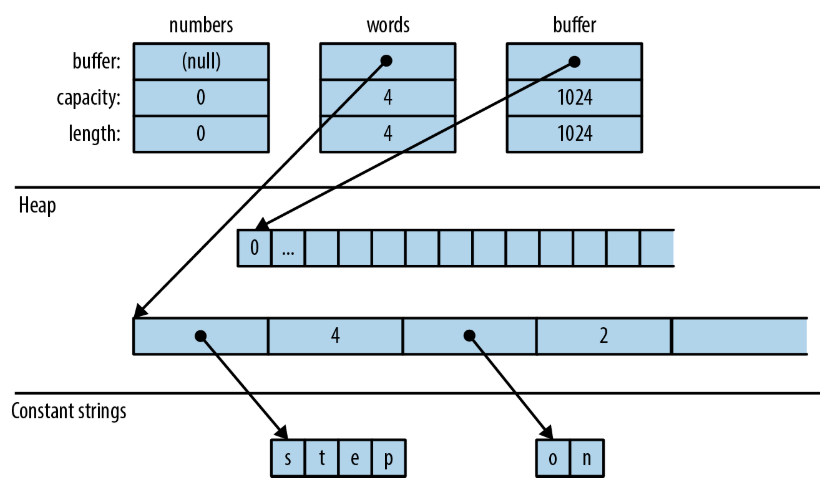
\includegraphics[width=0.9\textwidth]{../img/f16-1.png}
    \caption{vector的内存布局:words的每个元素是一个由指针和长度组成的\&str值}
    \label{f16-1}
\end{figure}

类似于所有集合,\texttt{Vec}实现了\texttt{std::iter::FromIterator},因此你可以对任何迭代器调用\texttt{.collect()}方法来创建一个vector,正如“\nameref{BuildColl}”中所述:
\begin{minted}{Rust}
    // 将一个其他集合转换成vector
    let my_vec = my_set.into_iter().collect::<Vec<String>>();
\end{minted}

\subsection{访问元素}
通过索引访问数组、切片或vector的元素非常直观:
\begin{minted}{Rust}
    // 获取一个元素的引用
    let first_line = &lines[0];

    // 获取一个元素的拷贝 
    let fifth_number = numbers[4];          // 需要Copy
    let second_number = lines[1].clone();   // 需要Clone

    // 获取一个切片的引用
    let my_ref = &buffer[4..12];

    // 获取一个切片的拷贝
    let my_copy = buffer[4..12].to_vec();   // 需要Clone
\end{minted}

当索引越界时所有这些方式都会panic。

Rust对数字类型很挑剔,vector也不例外。vector的长度和索引都是\texttt{usize}类型。尝试使用\texttt{u32}、\texttt{u64}、\texttt{isize}作为vector的索引会导致错误。必要时你可以使用\texttt{n as usize}来转换,见“\nameref{cast}”。

有几种方法提供了便捷地访问vector或切片的特定元素的方法(注意所有的切片方法都能用于数组和vector):
\codeentry{slice.first()}
\hangparagraph{返回\texttt{slice}的第一个元素的引用。返回类型是\texttt{Option<\&T>},因此如果\texttt{slice}为空时返回值为\texttt{None},不为空时返回值为\texttt{Some(\&slice[0])}}:
\begin{minted}{Rust}
    if let Some(item) = v.first() {
        println!("We got one! {}", item);
    }
\end{minted}

\codeentry{slice.last()}
\hangparagraph{和上边相似,不过返回最有一个元素的引用。}

\codeentry{slice.get(index)}
\hangparagraph{返回\texttt{slice[index]}的引用,如果存在的话。如果\texttt{slice}的元素数量小于\texttt{index+1},那么返回\texttt{None}}:
\begin{minted}{Rust}
    let slice = [0, 1, 2, 3];
    assert_eq!(slice.get(2), Some(&2));
    assert_eq!(slice.get(4), None);
\end{minted}

\codeentry{slice.first\_mut(), slice.last\_mut(), slice.get\_mut(index)}
\hangparagraph{与上面的类似,不过借用\texttt{mut}引用:}
\begin{minted}{Rust}
    let mut slice = [0, 1, 2, 3];
    {
        let last = slice.last_mut().unwrap();   // 最后一个元素类型:&mut i32
        assert_eq!(*last, 3);
        *last = 100;
    }
\end{minted}

因为以值返回\texttt{T}意味着移动它,因此访问元素的方法通常返回元素的引用。

一个例外是\texttt{.to\_vec()}方法,它获取拷贝:

\codeentry{slice.to\_vec()}
\hangparagraph{克隆整个切片,返回一个新的vector:}
\begin{minted}{Rust}
    let v = [1, 2, 3, 4, 5, 6, 7, 8, 9];
    assert_eq!(v.to_vec(),
               vec![1, 2, 3, 4, 5, 6, 7, 8, 9]);
    assert_eq!(v[0..6].to_vec(),
               vec![1, 2, 3, 4, 5, 6]);
\end{minted}
\hangparagraph{只有当元素可以拷贝时这个方法才可用,即\texttt{where T: Clone}}

\subsection{迭代}

